% Document class `report-template` accepts either project-plan or final-report option in
% []. This will change the title page as necessary.
% \documentclass[project-plan]{report-template}
\documentclass[final-report]{report-template}

% myself define
\usepackage{subcaption}


% Packages I use in my report.
\usepackage{graphicx}
\usepackage{amsmath}
\usepackage{blindtext}

% Directory where I saved my figures.
\graphicspath{{./figures/}}

% Metadata used for the title page - please modify.
\university{Imperial College London}
\department{Department of Earth Science and Engineering}
\course{MSc in Applied Computational Science and Engineering}
\title{Enhancing Commodity Price Predictions: Advanced Machine Learning Models for Copper Price Forecasting}
\author{Peifeng Tan}
\email{pt623@imperial.ac.uk}
\githubusername{acse-pt623}
\supervisors{Antony Sommerfeld\\
                Yves Plancherel}
\repository{https://github.com/acse-pt623/irp-pt623-external.git}

\begin{document}

\maketitlepage  % generate title page

% Abstract
\section*{Abstract}
Copper is an indispensable raw material in modern industry and life. It has been widely used in a variety of sectors including power electronics, household appliances, transportation and energy. However, as copper is both a commodity and financial product, its price forecasting becomes  exceptionally complex. Reference to other people's work, we are skeptical about using LSTM to predict daily price in financial time series forecasting, suspecting that the model cannot learned any meaningful information about this market at all, but only uses the price of the last date as the prediction result, which usually can achieve high performance on many evaluation criteria. However this is worthless in practical applications. This study will improve copper price forecasting by using advanced deep learning model and considering a range of factors. Therefore, we build two model including Multi-TCN-LSTM-Attention model and BNN-CNN-LSTM model to predict the next fifth day using previous information. Apart from that, we proposed a useful way of data augmentation using EMD decomposition to improve accuracy and robustness. 
% Finally, we use an advanced model - Autoformer to predict continuously next 5 days and 30 days, which has achieved the best performance.
% Introduction section
\section{Introduction}
\subsection{Background and Challenges}
Metals, including copper, are crucial raw materials and strategic resources for national economic development and the energy industry. Copper, in particular, is a key industrial material widely used in power electronics \cite{sun2018freezing} , household appliances, transportation, machinery manufacturing, and construction due to its excellent electrical conductivity, corrosion resistance, and versatility. Consequently, the global demand for copper has been on the rise.

Beyond its industrial applications, copper is also traded in commodity markets, giving it the attributes of a financial product.\cite{frankel2010determinants,behmiri2015role} This dual nature makes forecasting copper prices complex and challenging. The price of copper is influenced by a variety of factors, \cite{BUNCIC20151}including market supply and demand, political events, economic policies, and speculative behaviors, all of which contribute to its price volatility.

\subsection{Advanced Models and Their Limitations}
Accurate forecasting of copper price is crucial because of their significant impact on national economic development and the energy industry. In the past, researchers have employed various models such as ARIMA \cite{Asteriou2016ARIMAMA} to predict copper price. However, these linear model cannot effectively capture the nonlinear relationship in price changes. Machine learning methods such as NARX\cite{lin1996learning,diaconescu2008use,yan2013substructure}, ANN\cite{ZHANG2021102189,WANG2019101414}, KNN\cite{altman1992introduction}, SVM\cite{ZHANG2021102189}, XGBoost \cite{frigola2013integrated,breiman2001random} have also been applied with significant improvement.  Nevertheless, these models often struggle to capture the temporal dependencies effectively.

To address these problems, RNNs \cite{rumelhart1986learning1} were introduced into time series prediction, but suffer from the problem of gradient vanishing \cite{rumelhart1986learning} when dealing with long sequences. LSTM  \cite{hochreiter1997long,shi2015convolutional}and GRU networks, as an improvement over RNNs, can better capture long-time dependencies and have achieved remarkable results in time series predictions. 

However, after reproducing some simple LSTM models, I found that although they have achieved high performance in numerical evaluation indicators such as MSE, MAE, MAPE, MSPE and R2 score, they cannot be used in the real market. These model actually did not capture the underlying regulations of the market but only using today's price as the prediction of the next day. This result indirectly proves that the change in copper price has the characteristics of a random model making precise short-term predictions difficult.

\subsection{Research Objectives and Methodology}
This study aim to develop a robust model to forecast copper price that overcomes the limitations of existing models. The primary objectives are to incorporate a variety of influencing factors, including commodity and financial indicators, applying advanced machine learning models, such as LSTM, TCN \cite{lea2016temporalconvolutionalnetworksunified} and transformer encoder \cite{wen2023transformers}, Bayesian Neural Network (BNNs) \cite{item_79a95918d094486381eddd0e003bcd84}
 with self attention \cite{vaswani2017attention}, to improve model power to capture market regulation. 

To achieve these objectives, the study will collect and preprocess data from various sources and choose nine features which is correlated with copper price including copper price, Gold price , oil Brent price \cite{BILDIRICI2015397} , soybean price, tin price, Wheat price, silver price \cite{BILDIRICI2015397} , Commodity Research Bureau index and London Metal Exchange index. Inspired by recent research, we will utilize an multi-TCN-LSTM-Attention model \cite{CAO2019127} with EMD data augmentation, which combines Empirical Mode Decomposition (EMD) \cite{kim2009emd} , Temporal Convolutional Network (TCN), Long Short-Term Memory (LSTM) and Transformer Encoder Layer to better capture complex temporal dependencies and extract meaningful features. To incorporate various factors, we use self-attention model which has been proven to be successful in NLP work. Finally, we will use multi-task training approach to simultaneously predict nine market features to enforce model extracting underlying market regulation. This comprehensive approach aims to address the limitations of previous models and provide more practice way in financial market. Self-attention model provide more interpretable forecasts for copper prices.  

To further enhance the robustness of the forecasting model, we will incorporate a Bayesian Neural Network (BNN) approach, BNNs provide a significant advantage on financial forecasting by involving a  randomness bias to estimate uncertainty in the Copper Market. By learning a distribution of model parameters, it can provide a probabilistic forecast that reflect the real market uncertainties.

In our model, we use a TCN-LSTM model combined with BNN fully connected layers. This setup allows the model to learn the underlying distribution of the market features and produce more reliable predictions with associated confidence intervals. 

% However, both of previous methods can only the predict of a single day. Since the price of a  single day has the characteristics of random walk, the single day prediction cannot reflect the accuracy and stability of the model in actual applications and lacks practical application significance. Therefore, we refer to the project Autoformer \cite{wu2021autoformer} model which is depending on the transformer and signal decomposition methods to try to achieve continuous prediction of 5-day and 30-day prices, hoping to reflect the trend through continuous time prediction, so as to prove its value in practical applications.

\section{Methods}

\subsection{Data Processing}

\subsubsection{Data Collection}
To forecast copper price, we collected dataset from 4 February 1994 to 1 July 2024. The data sources includes

\begin{enumerate}
    \item \textbf{Historical commodity price Data: } historical prices of copper, gold, silver, tin and zinc which are copper-related metal, Crude oil price , Brent oil price, natural gas price which are related energy prices with copper production and industry production,
    \item \textbf{Financial Market Indicators : }
    \begin{enumerate}
        \item Dow Jones Industrial Average (DJIA)
        \item S\&P 500 Index
    \end{enumerate}
    \item \textbf{Composite Indices :}
    \begin{enumerate}
        \item Commodity Research Bureau Index (CRB Index)
        \item Goldman Sachs Commodity Index (GSCI)
        \item London Metal Exchange Index (LME Index)
        \item Shanghai Stock Exchange Consumer Commodity Index (SSE Consumer Commodity Index)
    \end{enumerate}  
\end{enumerate} 

After collecting the dataset, we processed with data cleaning and preprocessing for each features to ensure the quality and consistency of the inputs. This process included removing missing values and combining data based on date.
\begin{figure}[h]
    \centering
    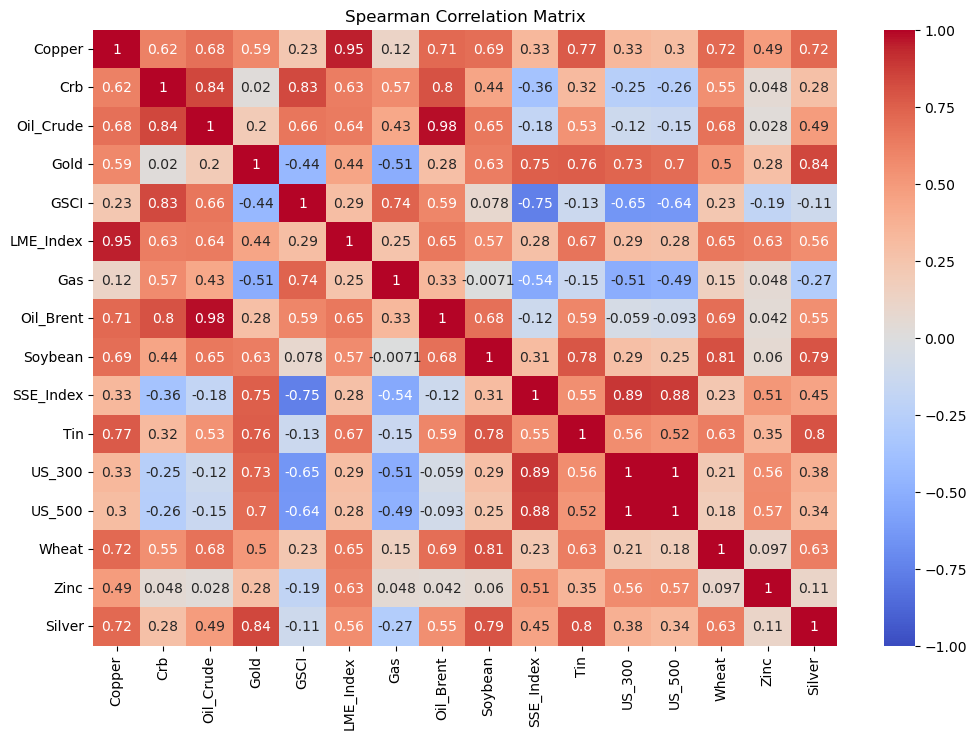
\includegraphics[width=1\linewidth]{figures/factors_spearman.png}
    \caption{Spearman coefficient of factors}
    \label{fig:spearman}
\end{figure}
To avoid introducing irrelevant features that could potentially polluted the model result,  we use Spearman's rank correlation \autoref{fig:spearman} which measures monotonic relationships.  This method was chosen for its robustness in capturing both linear and non-linear relationships between the features and the target variable-copper prices. 

Based on the Spearman correlation \cite{spearman2008} analysis result, we selected the nine features that exhibited a correlation coefficient greater than 0.6 with copper price. These features will be used as input of our model, guaranteeing that only relevant features would be utilized for forecasting.\cite{zhong2019time}

\subsubsection{Data Preprocessing}
Data preprocessing is crucial to ensure the robust and quality of the model.  The preprocessing steps include: 
\begin{itemize}
    \item Handling missing values: Imputation or removal of missing data points.
    \item     Feature extraction: Using Empirical Mode Decomposition (EMD) to decompose time series data into intrinsic mode functions (IMFs) and remove the first one.~\autoref{fig:Copper_EMD}
    \item Normalization: Scaling data to a standard range to improve model convergence.
\end{itemize}
\begin{figure}[h]
    \centering
    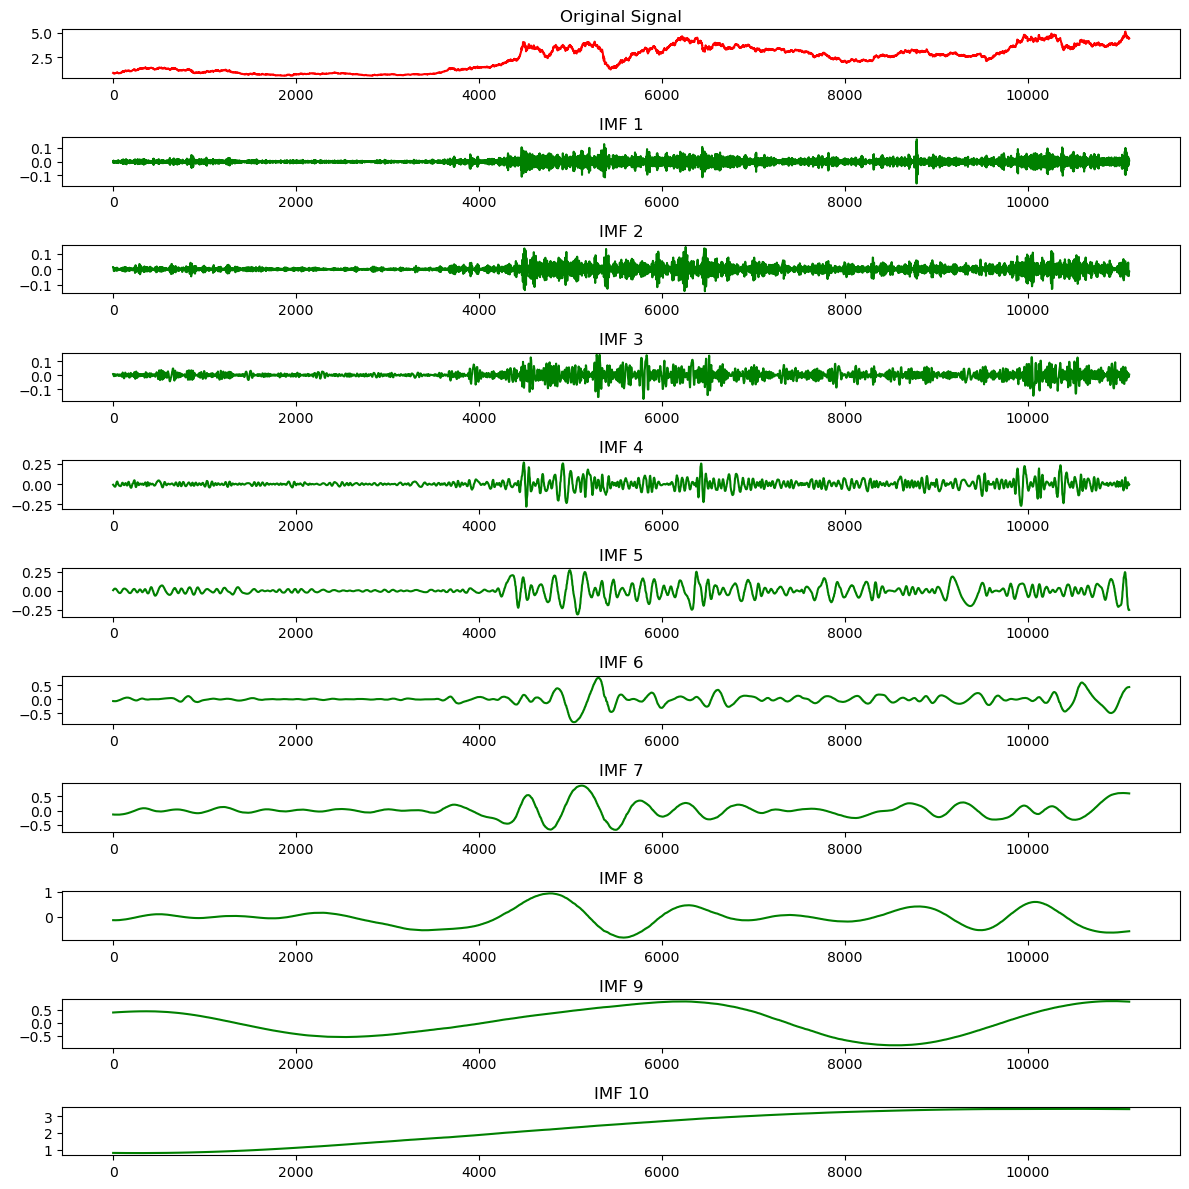
\includegraphics[width=0.5\linewidth]{figures/EMD_copper.png}
    \caption{EMD result of Copper price}
    \label{fig:Copper_EMD}
\end{figure}
\subsubsection{\textbf{Data Augmentation}}
Data augmentation is an essential technique used to enhance the robustness and generalization ability of the model. In this study, we applied a novel data augmentation method based on Empirical Mode Decomposition (EMD). The augmentation process involves the following steps:
\begin{itemize}
    \item \textbf{EMD Decomposition}: The original time series data is decomposed into intrinsic mode functions (IMFs) using EMD. 
    \item \textbf{Label Variation}: A new set of training labels is created by removing the first one or two IMF components. 
    \item \textbf{Data Combination}: The various datasets generated through this process are combined into a single training set. This approach not only increases the overall dataset size but also introduces a range of label variations that help prevent the model from overfitting to specific noise patterns in the data.
\end{itemize}

The purpose of this augmentation is threefold:
\begin{enumerate}
    \item \textbf{Avoiding Overfitting}: By providing multiple label sets for the same time period, the model is discouraged from memorizing specific data points, such as using the actual value of today's price as a direct prediction for the fifth day. Instead, it is forced to learn more generalized patterns.
    \item \textbf{Learning a Balanced Representation}: The model is encouraged to learn an average representation between the actual values and the noise-reduced values. This results in predictions that better reflect the underlying trends, rather than being overly influenced by daily random fluctuations.
    \item \textbf{Increasing Data Volume}: Augmentation effectively increases the amount of training data available, which is particularly beneficial for complex models like Bayesian Neural Networks (BNNs) that require more data to accurately capture the stochastic nature of financial time series.
\end{enumerate}

Experimental results have demonstrated that this data augmentation technique significantly improves the model's generalization ability. The augmented model shows better performance on the validation set, suggesting that it is more capable of capturing the inherent randomness and trends in the data. Furthermore, this method aligns well with the strengths of Bayesian Neural Networks, allowing them to more effectively capture and represent the distribution of daily random fluctuations.

\subsection{Model Construction}

\subsubsection{\textbf{Empirical Mode Decomposition (EMD)}}
Empirical Mode Decomposition (EMD) is a method used to decompose a time series into a set of Intrinsic Mode Functions (IMFs) according to different frequency.  Each IMF represents a simple oscillatory mode components within the data, which is particularly useful for analyzing non-linear and non-stationary signals. In this study, EMD is applied to the copper price time series data to extract main trend part and remove random noise part. \autoref{fig:Copper_EMD} We remove the first n IMF component and reassemble other parts to get a more stable price trend as new labels.

\subsubsection{\textbf{Temporal Convolutional Networks (TCN)}}
Temporal Convolutional Networks (TCN) are a type of convolutional neural network designed for sequence modeling tasks. Unlike traditional convolutional networks, TCNs use causal convolutions and dilations to capture long-range dependencies in time series data.  It use 1D Convolutional Network with padding at the end to ensure that the shape of output is same as input shape.  Apart from that,  dilation can be used to expand the receptiive field of kernels.  In our model, TCNs are employed to capture the temporal dependencies within the decomposed components obtained from EMD, providing a robust foundation for downstream modeling.  We only use one layer TCN model to capture trend change in past features.  To be specific, we build a block model called ResidualBlock\autoref{fig:tcn block} which includes two convolutional network with ReLU activation and adding original input to avoid gradient vanishing and exploding. \cite{lea2016temporalconvolutionalnetworksunified}
\begin{figure}[h]
    \centering
    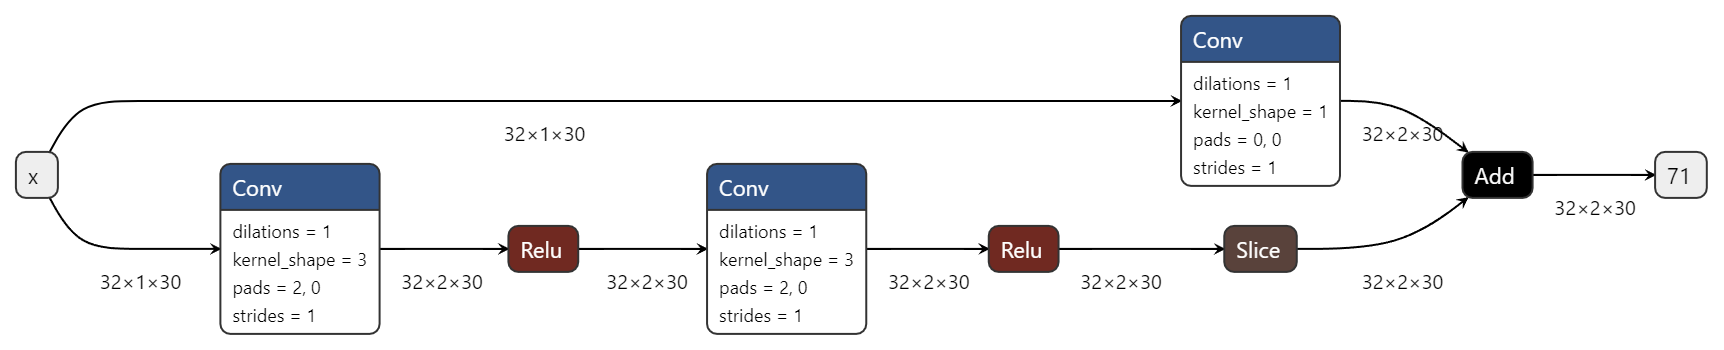
\includegraphics[width=1\linewidth]{figures/simple_residualblock.onnx.png}
    \caption{TCN Residual Block}
    \label{fig:tcn block}
\end{figure}
\subsubsection{\textbf{Long Short-Term Memory (LSTM) Networks}}
Long Short-Term Memory (LSTM) networks are a development of recurrent neural network (RNN) \cite{rumelhart1986learning} designed to capture long-term dependencies in sequential data. It use gate structures involving input-gate, forget gate and output-gate.  LSTMs effectively avoid  vanishing gradient issues that traditional RNNs face. In our model, LSTM networks are used to model the long-term dependencies within the time series data for each of nine features, enabling the prediction of future copper prices based on historical trends. 
\begin{equation}
f_t = \sigma(W_f \cdot [h_{t-1}, x_t] + b_f)
\end{equation}
\begin{equation}
i_t = \sigma(W_i \cdot [h_{t-1}, x_t] + b_i)
\end{equation}
\begin{equation}
o_t = \sigma(W_o \cdot [h_{t-1}, x_t] + b_o)
\end{equation}
\subsubsection{\textbf{Self-Attention and Transformer Encoder Layer}}
The self-attention mechanism is a key component of the Transformer encoder\autoref{fig:encoder layer}, which allows the model to capture useful information among different features when making predictions. This mechanism improves the model's ability to measure relationships of elements. In our model, we use this part to exchange deep characteristic of nine features, further enhancing the model's interpretability and performance.\cite{vaswani2017attention,li2019enhancing,wen2023transformers}
\begin{figure}[h]
    \centering
    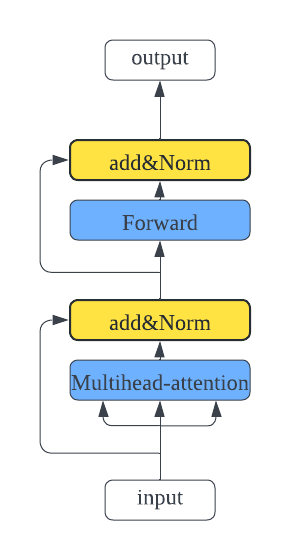
\includegraphics[width=0.5\linewidth, height=0.5\textwidth]{figures/multiattention.png}
    \caption{Transformer Encoder Layer}
    \label{fig:encoder layer}
\end{figure}
\subsubsection{\textbf{Bayesian Neural Networks (BNN)}}
Bayesian Neural Networks (BNN) extend traditional neural networks by setting a prior distribution over the network's weights, rather than assuming a single fixed value. This approach allows BNNs to estimate the predictions with the uncertainty associated. In the context of financial forecasting, where market behavior is often influenced by unpredictable factors, BNNs provide a probabilistic framework that better captures this uncertainty.

In our model, after processing the features through the CNN-LSTM architecture, the linear layers is replaced with a Bayesian Linear Layers. This layer outputs a distribution for prediction rather than a single deterministic value. The advantage of this model is that it produces a range of outcomes with associated distribution, which is crucial for financial market with random walk model. 

This model depends on the Bayesian inference which is a statistical method updating the probability estimate for a hypothesis as more evidence and observed information becomes available. It combines prior distribution with observed data to form a posterior distribution. 
\begin{equation}
p(w \mid D) = \frac{p(D \mid w) p(w)}{p(D)} = \frac{p(D \mid w) p(w)}{\int_{w'} p(D \mid w') p(w') dw'}
\end{equation}
To train this model, the core goal is to learn the posterior distribution of the parameters \(p(D \mid w)\), where \(w\) represents the parameters and \(D\) is the observed data. Since directly computing this posterior distribution is usually infeasible, BNNs use some techniques like variational inference to approximate this distribution.\cite{item_79a95918d094486381eddd0e003bcd84}

\subsubsection{\textbf{Proposed EMD-TCN-LSTM Model with Self-Attention}}
The proposed model, multi-TCN-LSTM-Attention model, is designed to effectively capture and model temporal dependencies in time series data and relationships among all features. The model uses Empirical Model Decomposition model to create more label, which remove random part. This is a kind of data augmentation and have been approved useful. Then, they are fed into parallel Temporal Convolutional Network layers to extract temporal features from each features independently, which are then processed by Long Short-Term Memory (LSTM) networks to capture time dependencies. The outputs of nine TCN-LSTM model are passed into a Self-Attention mechanism, which dynamically weights the importance of different features and communicate with each others, enabling the model to focus on the most relevant parts of the data.\autoref{fig:mixed-model} Finally, using individual fully connected  nine individual layers (FC) aggregate the outputs from the attention mechanism to generate the final nine predictions. 
\begin{figure}[h]
    \centering
    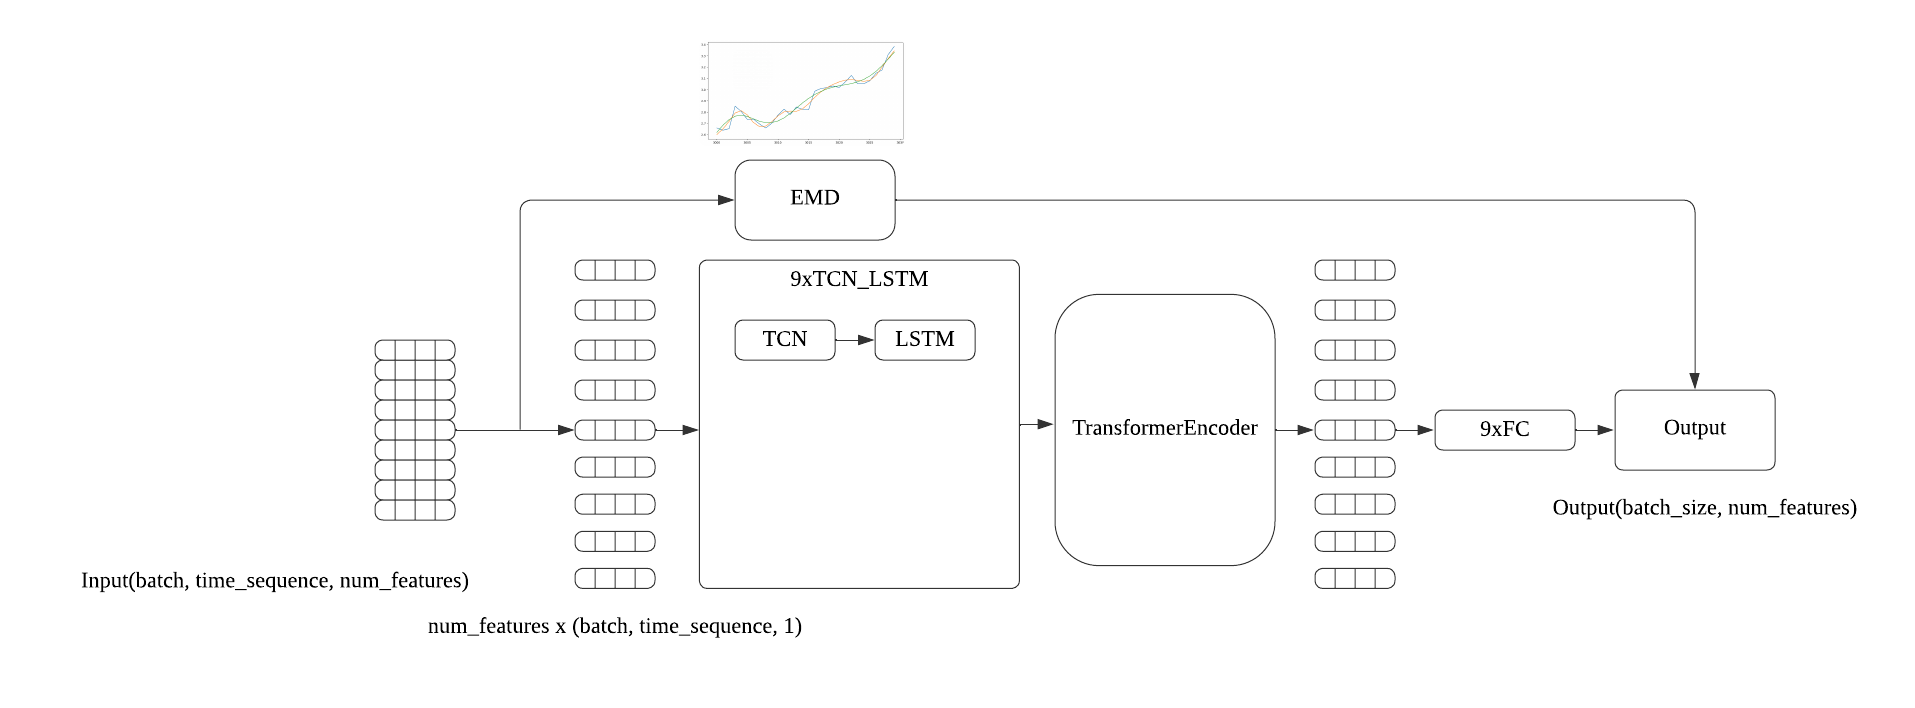
\includegraphics[width=1\linewidth]{figures/mixed_model.png}
    \caption{EMD-TCN-LSTM with Attention Model}
    \label{fig:mixed-model}
\end{figure}

% \subsection{Autoformer: A Novel Architecture for Time Series Forecasting}\cite{wu2021autoformer}
% Autoformer is a new architecture designed for time series forecasting based on the Transformer structure. Its purpose is to address the limitations of traditional Transformer models in processing long sequences and effectively capturing temporal patterns. Unlike the standard Transformer, which relies on an attention mechanism that grows quadratically with the length of the sequence, Autoformer introduces two key innovations: an autocorrelation mechanism and a decomposition block.
% \begin{figure}
%     \centering
%     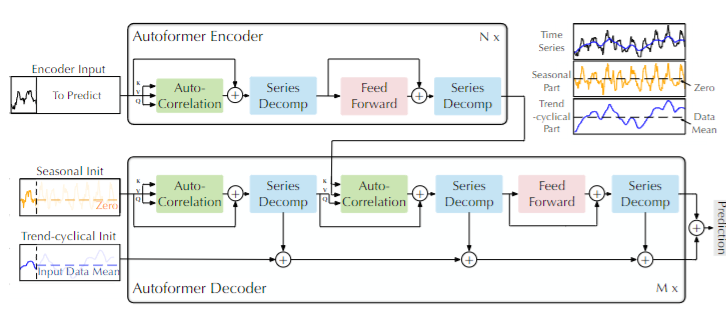
\includegraphics[width=1\linewidth]{figures/Autoformer.png}
%     \caption{AutoFormer Model\cite{wu2021autoformer}}
%     \label{fig:autoformer}
% \end{figure}

% The autocorrelation mechanism replaces the traditional standard sub-attention mechanism. By identifying and exploiting the autocorrelation of time series data, the Autoformer can focus on the most relevant lag time, reduce computational complexity, and increase the model's ability to capture long-term dependencies. In addition, the model makes full use of the decomposition function in signal processing to decompose the input time series into trend and seasonal components. This helps the model directly learn the underlying pattern, which is similar to the Empirical Mode Decomposition (EMD) we considered earlier, greatly improving accuracy.

% Compared with traditional architectures such as LSTM or TCN, Autoformer is more efficient when processing long sequences and provides better interpretability by explicitly modeling temporal dependencies. This makes Autoformer particularly suitable for application in complex time series forecasting tasks where capturing long-term dependencies is critical.

\section{Experimental Setup}

\subsection{Experiment Objectives}
The primary objective of the experiments is to systematically evaluate and compare the effectiveness of several machine learning models in predicting copper prices. Specifically, the experiments focus on the following tasks:

\begin{itemize}
    \item \textbf{The Fifth Day Copper Price Prediction:} Evaluating how well the models can forecast the copper price five days ahead, which is a more challenging task given the increased forecast horizon.
    % \item \textbf{Continuous Five Days and Thirty Days Prediction:} Evaluating how well the AutoForemer can forecast the copper price continuously for 5 and 30 days.
\end{itemize}

The models under comparison include a basic Long Short-Term Memory (LSTM) network, a Convolutional Neural Network combined with LSTM (CNN-LSTM) with multiple input features, the Temporal Convolutional Network, LSTM, Self-Attention (Multi-TCN-LSTM-Attention) model, LSTM model with Bayesian Layer and CNN-LSTM Beyasian Layer.

\subsection{Model Configurations}
In this subsection, we provide detailed descriptions of the configuration and architecture of each model used in the experiments:

\subsubsection{\textbf{LSTM Model}}
The LSTM model serves as the baseline for comparison. It is configured with the following specifications:
\begin{itemize}
    \item \textbf{Input Sequence}: The model takes a sequence of past copper prices as input. The length of this sequence (i.e., the look-back period) is set to 30 days, meaning the model uses the past 30 days of prices to predict the next day’s price.
    \item \textbf{LSTM Layer}: The model consists of 2 LSTM layers with 512 hidden units. This layer is responsible for capturing the temporal dependencies in the data.
    \item \textbf{Output}: The output is a single value representing the predicted copper price for the next day or the price five days ahead, depending on the task.
    \item \textbf{Activation and Optimization}: The model is optimized using the Adam optimizer with a learning rate of 0.0001 and using CosineAnnealingWarmRestarts scheduler to adjust learning rate.
\end{itemize}

\subsubsection{\textbf{CNN-LSTM Model (Multiple Inputs)}}
This model extends the single-input CNN-LSTM by incorporating additional features:
\begin{itemize}
    \item \textbf{Input Features}: The model takes nine different features as inputs, including copper price, related metal prices (gold, silver, tin,), energy prices (crude oil, Brent oil), and financial indices.
    \item \textbf{Separate CNN Layers}: Each input feature is processed independently by a separate 1D convolutional layer, configured similarly to the single-input CNN-LSTM model.
    \item \textbf{Feature Combination}: The output of each CNN layer is concatenated and fed into an LSTM layer with one layer and 512 units. This configuration allows the model to capture both temporal dependencies and interactions between different features.
    \item \textbf{Output}: The model provides predictions for the next day's copper price and the price five days ahead.
\end{itemize}

\subsubsection{\textbf{Multi-TCN-LSTM-Attention Model}}
The proposed EMD-TCN-LSTM-Attention model is designed to leverage the strengths of multiple techniques for improved forecasting accuracy:
\begin{itemize}
    \item \textbf{Empirical Mode Decomposition (EMD)}: The historical copper price series is first decomposed into several Intrinsic Mode Functions (IMFs) using EMD. This step aims to separate the underlying trends from random noise.
    \item \textbf{TCN Layer}: The decomposed components are processed by a Temporal Convolutional Network (TCN) layer, which captures both short-term and long-term dependencies in the data. The TCN layer is configured with dilated convolutions to ensure a large receptive field.
    \item \textbf{LSTM Layer}: The output from the TCN layer is fed into an LSTM layer with 512 units, which further models the temporal dependencies across the decomposed signals.
    \item \textbf{Self-Attention Mechanism}: A self-attention layer is applied to the outputs of the LSTM layer to dynamically weigh the importance of different features and time steps, allowing the model to focus on the most relevant parts of the data. The number of encoder layer is one.
    \item \textbf{Output}: Finally, the output from the self-attention mechanism is passed through a series of fully connected layers to generate the final price predictions.
\end{itemize}

\subsubsection{\textbf{CNN-LSTM-BNN Model (Bayesian Neural Network)}}
This model combines the strengths of CNN, LSTM, and Bayesian Neural Networks (BNN) to enhance the robustness of the forecasting:
\begin{itemize}
\item \textbf{Input Features}: The model processes nine different input features, including copper price, related metal prices (gold, silver, tin), energy prices (crude oil, Brent oil), and financial indices.
\item \textbf{CNN Layers}: All input features are  processed by a 1D convolutional layer. The CNN layers extract local patterns and features from the input sequences.
\item \textbf{LSTM Layer}: The outputs of the CNN layers are concatenated and fed into an LSTM layer with 512 units, allowing the model to capture temporal dependencies across different features.
\item \textbf{Bayesian Fully Connected Layers}: The output from the LSTM layer is passed through a series of three Bayesian fully connected (BayesLinear) layers. These layers model the uncertainty in predictions by learning distributions over weights, making the model more resilient to overfitting and better at capturing market uncertainties.
\item \textbf{Output}: The model generates predictions for the next day's copper price and the price five days ahead, incorporating the uncertainty captured by the Bayesian layers.
\end{itemize}

\subsubsection{\textbf{LSTM-BNN Model (Bayesian Neural Network})}
The LSTM-BNN model aims to leverage the temporal modeling capabilities of LSTM and the uncertainty estimation of Bayesian Neural Networks:
\begin{itemize}
\item \textbf{Input Features}: Similar to the CNN-LSTM-BNN model, this model takes nine input features related to copper and other market factors.
\item \textbf{LSTM Layer}: The input features are directly fed into an LSTM layer with 512 units, which captures the temporal dependencies in the data across all input features.
\item \textbf{Bayesian Fully Connected Layers}: The LSTM output is then passed through three Bayesian fully connected (BayesLinear) layers. These layers help the model to quantify uncertainty in its predictions, providing a distribution over the possible future copper prices.
\item \textbf{Output}: The final output includes predictions for the next day's copper price and the price five days ahead, with the Bayesian layers ensuring the predictions reflect the inherent uncertainty in the market data.
\end{itemize}

% \subsubsection{\textbf{Autoformer Model}}
% The Autoformer model is designed to effectively capture temporal dependencies and long-term patterns in time series data and ca be used to predict ontinuous days. The following outlines the key components and experimental setup for the Autoformer model:

% \begin{itemize}
% \item \textbf{Input Features}: The input features for the Autoformer model include both temporal features and market factors. The time features include \textit{month\_sin}, \textit{month\_cos}, \textit{day\_of\_week\_sin}, \textit{day\_of\_week\_cos}, and market-related features such as \textit{Crb}, \textit{Gold}, \textit{LME\_Index}, \textit{Oil\_Brent}, \textit{Soybean}, \textit{Tin}, \textit{Wheat}, and \textit{Silver}. 

% \item \textbf{Training Phase Inputs}:
% \begin{itemize}
%     \item \textbf{Past Values (\textit{x\_batch})}: The actual past values of copper prices.
%     \item \textbf{Future Values (\textit{y\_batch})}: The target future values of copper prices for prediction.
%     \item \textbf{Past Time Features (\textit{x\_time})}: Includes the temporal features and market factors for the past time steps. The market factors in this input are the actual known values.
%     \item \textbf{Future Time Features (\textit{future\_time})}: Includes the temporal features and market factors for the future time steps. While the temporal features are naturally determined, the market factors are filled using the last known values from the past.
%     \item \textbf{Past Observed Mask (\textit{x\_mask})}: A mask indicating which past values are observed and should be considered during training.
% \end{itemize}

% \item \textbf{Output}: The final output consists of predictions for the future copper prices.

% \end{itemize}

% \subsection{Experiment Comparison}
% The performance of each model is evaluated using several key metrics:
% \begin{itemize}
%     \item \textbf{Mean Squared Error (MSE)}: Measures the average squared difference between the predicted and actual prices. 
%     \item \textbf{Mean Absolute Error (MAE)}: Represents the average absolute difference between the predicted and actual prices. 
%     \item \textbf{R-squared (R²)}: Indicates the proportion of variance in the dependent variable that is predictable from the independent variables. It provides insight into the overall fit of the model.
%     \item \textbf{Mean Absolute Percentage Error (MAPE)}: Measures the average absolute percentage difference between the predicted and actual prices. It is useful for understanding the prediction error in relative terms, which can be easier to interpret, especially when comparing models.
%     \item \textbf{Mean Squared Percentage Error (MSPE)}: Represents the average squared percentage difference between the predicted and actual prices. Similar to MAPE, but more sensitive to large errors, providing a stricter measure of predictive accuracy.
% \end{itemize}

\subsection{Implementation Details}
This section provides technical details about the implementation, including:
\begin{itemize}
    \item Software and libraries used: Python, Pytorch, Torchbnn
    \item Hardware:  NVIDIA GeForce RTX 3060
\end{itemize}

\section{Results}

\subsection{Model Performance Overview}
\autoref{tab:performance_overview} summarizes the performance of all models based on the evaluation metrics described above. Each model's accuracy is compared using Mean Squared Error (MSE), Mean Absolute Error (MAE), R-squared (R²), Mean Absolute Percentage Error (MAPE), and Mean Squared Percentage Error (MSPE).
\begin{table}[h]
\centering
\caption{Performance Overview of Different Models 5days}
\label{tab:performance_overview}
\resizebox{\textwidth}{!}{
\begin{tabular}{lccccc}
\hline
\textbf{Model} & \textbf{MSE} & \textbf{MAE} & \textbf{R²} & \textbf{MAPE (\%)} & \textbf{MSPE (\%)} \\
\hline
LSTM &  0.0256& 0.1198& 0.8325&  2.9481& 0.1508\\
\hline
CNN-LSTM & 0.0225& 0.1148& 0.8529& 2.8511& 0.1358\\
\hline
EMD-TCN-LSTM-Attention & 0.0188& 0.1049& 0.8766& 2.6026& 0.1148\\
\hline
\textbf{EMD-TCN-LSTM-Attention} (Data Augmentation) & 0.0185& 0.1037 & 0.8788 & 2.5766 & 0.1127 \\
\hline
\textbf{BNN-CNN-LSTM}(Data Augmentation) & 0.0214 & 0.1096 & 0.8578 & 2.7124 & 0.1283 \\
\hline
BNN-LSTM(Data Augmentation) & 0.0343 & 0.1456 & 0.7722 & 3.6762 & 0.2149 \\
\hline
\end{tabular}}
\end{table}

As illustrate in the table, all advanced models significantly outperform the baseline LSTM model across all evaluation metrics. Notably, models with CNN or TCN, such as the CNN-LSTM, BNN-CNN-LSTM, show marked improvements in performance compared to the LSTM model. This highlights the effectiveness of CNNs in capturing loacl patterns within data, 

Among the models, the Multi-TCN-LSTM-Attention model and BNN-CNN-LSTM model stand out as the best performers. The Multi-TCN-LSTM-Attention model, in particular, demonstrates strong performance across all metrics, even without data augmentation. When data augmentation is applied, its performance further improves, achieving an MSE of 0.01855 and an R² of 0.8788. This underscores the model's capability to effectively capture complex temporal dependencies in the time series data. 

Overall, these results indicate that employing more sophisticated neural network architectures and data augmentation techniques can effectively enhance the accuracy and robustness of copper price forecasting models, providing more valuable and deeper insights for time series prediction in financial market.
\begin{table}[h]
\centering
\caption{Model Complexity Comparison}
\label{tab:model_complexity}
\resizebox{\textwidth}{!}{
\begin{tabular}{lcc}
\hline
\textbf{Model} & \textbf{Parameters (Millions)} & \textbf{Training Time (seconds/epoch)} \\
\hline
LSTM & 0.062M& 0.2427\\
\hline
CNN-LSTM & 3.258M& 1.8163\\
\hline
EMD-TCN-LSTM-Attention & 12.9M & 2.091\\
\hline
BNN-CNN-LSTM & 0.075M& 1.2429\\
\hline
BNN-LSTM & 0.073M& 0.7939\\
\hline
\end{tabular}}
\end{table}
\textbf{Training Efficiency}: While the more complex models generally offer better performance, this comes at the cost of increased computational requirements. As shown in Table \autoref{tab:model_complexity}, the training time per epoch increases with model complexity, particularly for BNN-based models due to their inherent complexity in managing probabilistic layers.

% \begin{figure}[h]
%     \centering
%     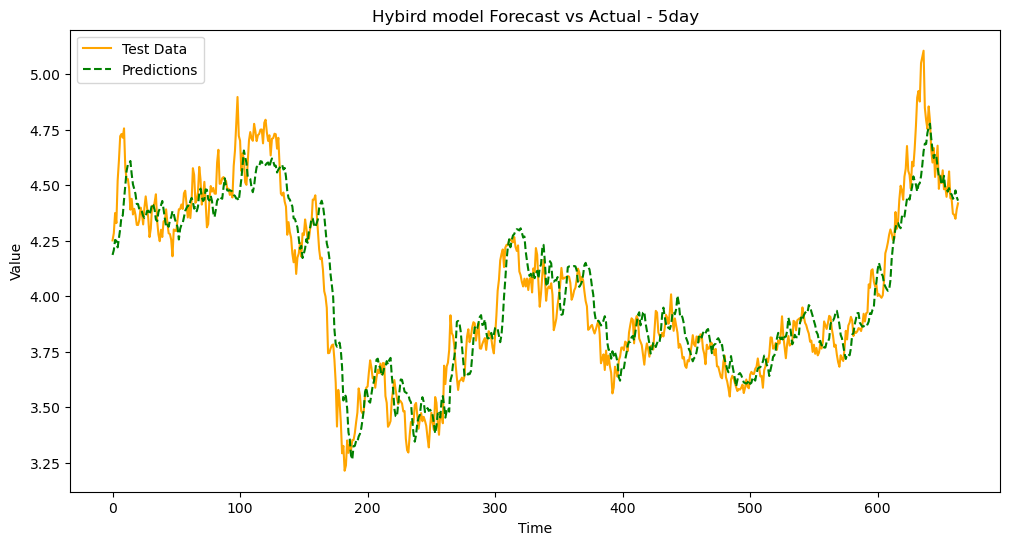
\includegraphics[width=0.7\linewidth]{figures/lstm_prediction_curve.png}
%     \caption{LSTM Model Prediction Curve}
%     \label{fig:lstm_prediction_curve}
% \end{figure}
% \begin{figure}[h]
%     \centering
%     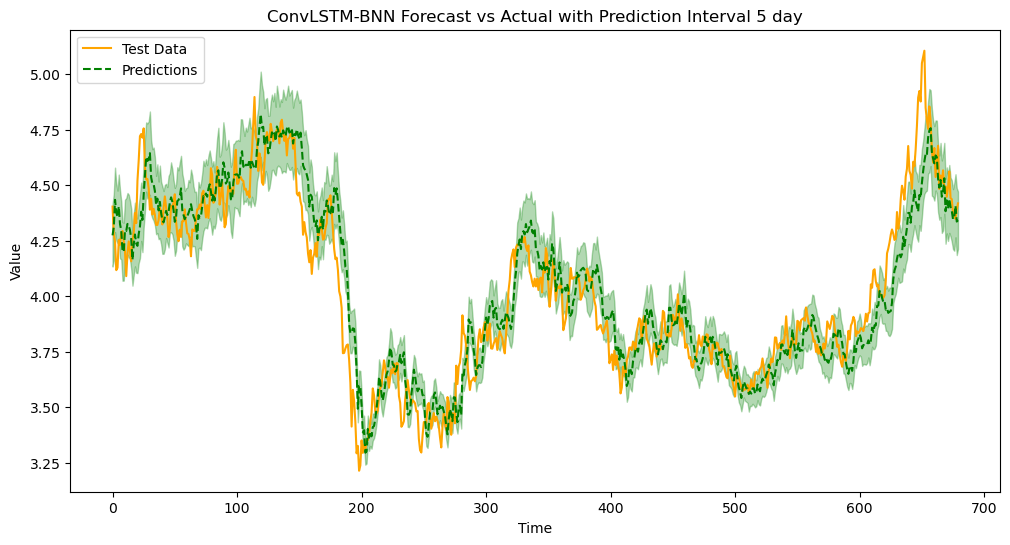
\includegraphics[width=0.7\linewidth]{figures/bnn_prediction_curve.png}
%     \caption{BNN-CNN-LSTM Model Prediction Curve}
%     \label{fig:bnn_prediction_curve}
% \end{figure}
\begin{figure}[h]
    \centering
    \begin{subfigure}[b]{0.48\linewidth}
        \centering
        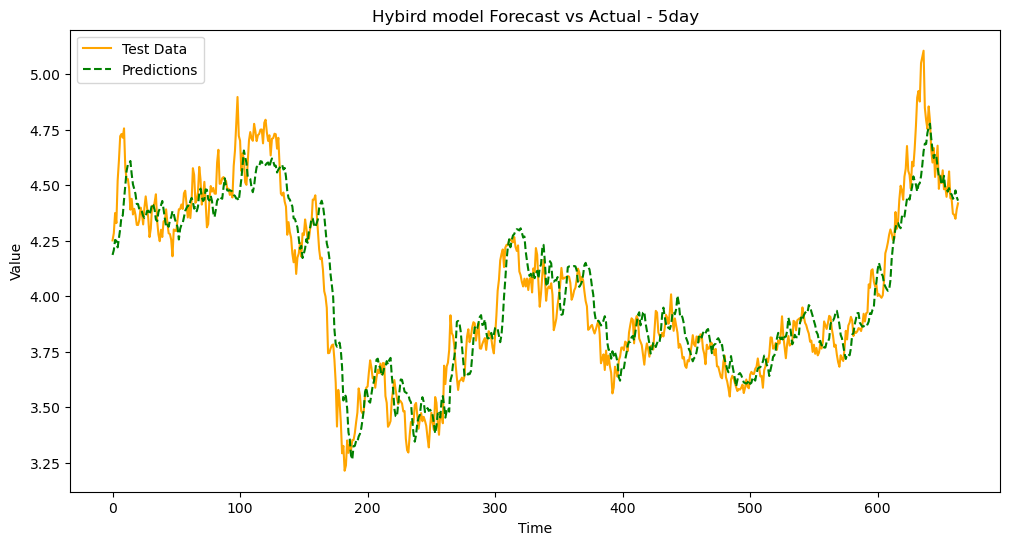
\includegraphics[width=\linewidth]{figures/lstm_prediction_curve.png}
        \caption{LSTM Model Prediction Curve}
        \label{fig:lstm_prediction_curve}
    \end{subfigure}
    \hfill
    \begin{subfigure}[b]{0.48\linewidth}
        \centering
        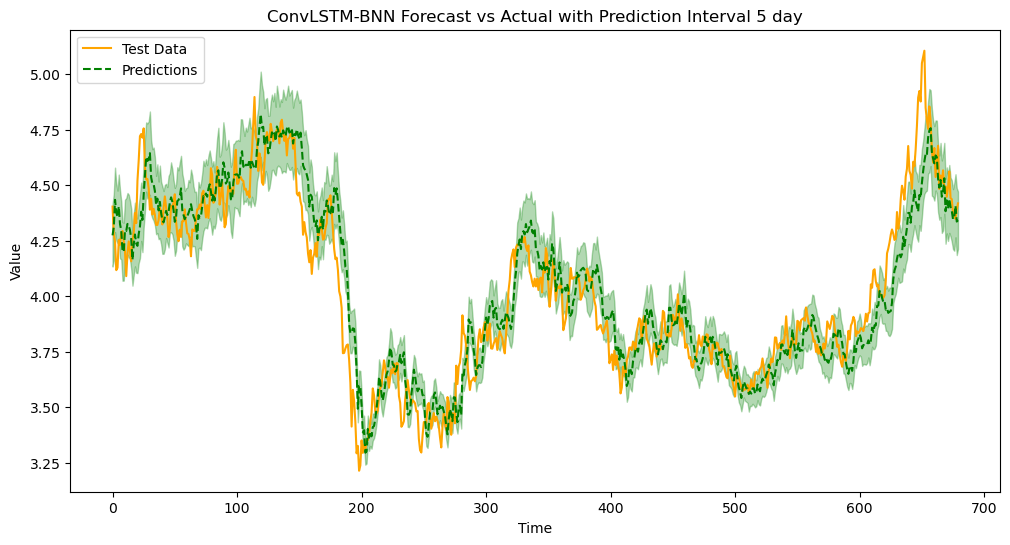
\includegraphics[width=\linewidth]{figures/bnn_prediction_curve.png}
        \caption{BNN-CNN-LSTM Model Prediction Curve}
        \label{fig:bnn_prediction_curve}
    \end{subfigure}
    \caption{Comparison of Prediction Curves for Different Models}
    \label{fig:combined_prediction_curves}
\end{figure}

\subsection{Prediction Curves}
To further illustrate the performance of the best two models, \autoref{fig:combined_prediction_curves} show the prediction curves of the Multi-TCN-LSTM-Attention model and BNN-CNN-LSTM models respectively.

\section{Discussion}

\begin{figure}[h]
    \centering
    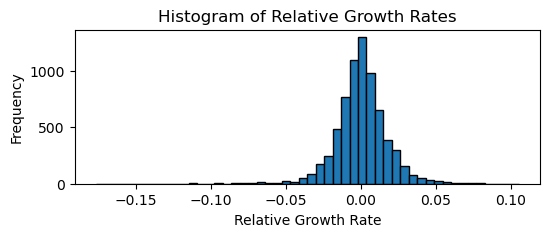
\includegraphics[width=0.8\linewidth]{figures/relative_incrrease.png}
    \caption{Relative Growth Rate}
    \label{fig:relative growth rate}
\end{figure}
\subsection{The Random Walk Model in the Copper Market}
Copper prices often present characteristic of a random walk, a theory in financial economics suggesting that stock prices and market prices include a random and unpredictable part. Empirical evidence supports that copper prices are highly fluctuating and have a random walk, making them difficult to predict with traditional time series models. The LSTM model, although powerful for capturing temporal dependencies, might struggle in this situation. The model often learns to use the current day's price as a naive prediction for the next day's price, rather than capturing underlying market trends. In our experiments, we can see that LSTM often presents time lag with true price and I also check the histogram of relative grown rates. \autoref{fig:relative growth rate} It is a very standard normal distribution which also support the random walk assumption. So, the best prediction of next day price is today 's price in random walk model.

\subsection{Addressing Randomness with EMD Decomposition}
Fortunately, we can predict the trend of Copper price instead of exact price value. To remove the effects of daily randomness in copper prices, we applied Empirical Mode Decomposition (EMD) to preprocess the data. \autoref{fig:EMD data augmentation} EMD decomposes the price series into several Intrinsic Mode Functions (IMFs). By removing the high-frequency IMFs, we aim to reduce the random noise and retain the more stable price trend. However, a limitation of this approach is that EMD requires process to the entire dataset for decomposition, leading to potential data leakage and making it challenging to ensure that the model is learning meaningful market information rather than capture simple regression information with data after removing noise.
\begin{figure}
    \centering
    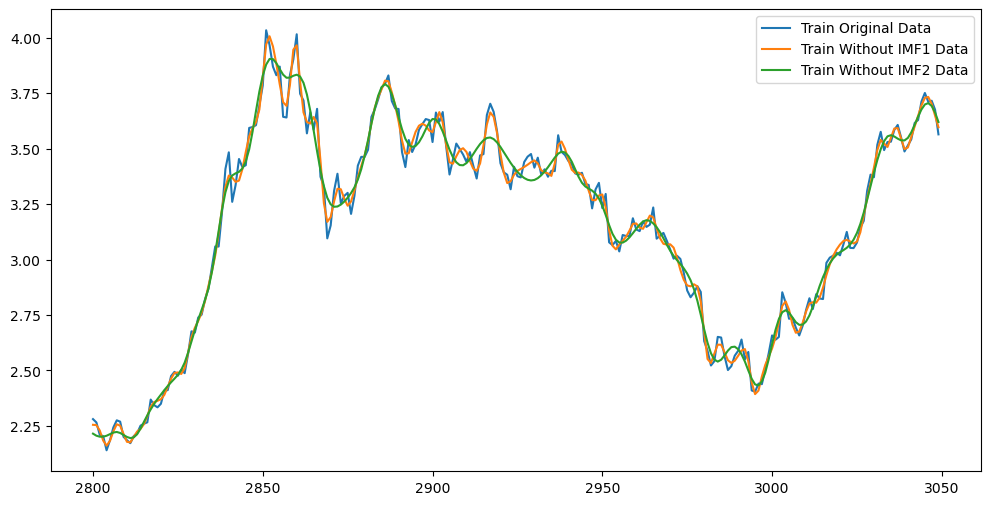
\includegraphics[width=1\linewidth]{figures/data_augmentation.png}
    \caption{Data Augmentation using EMD}
    \label{fig:EMD data augmentation}
\end{figure}
\subsection{Combining Data Augmentation with EMD Decomposition}
To overcome the limitations of direct EMD application as input dataset, we implemented a data augmentation strategy where different IMF components were used to generate multiple training labels. This approach helps prevent the model from simply using today's price as the predicted value for future prices. Additionally, this method enforces the model to learn an average behavior that balances both long-term trends and daily randomness, thus improving the model's generalization ability. 

The \autoref{tab:performance_overview} illustrates the significant impact of data augmentation on model performance. The model using data augmentation, specifically the Multi-TCN-LSTM-Attention, achieved better validation performance. This method, by generating different training label using EMD method, enables the model to better capture trends of the copper market, improving generalization and reducing the risk of overfitting. Our experiments demonstrate that this data augmentation strategy enhances the model's performance on the validation dataset, particularly for Bayesian Neural Networks (BNNs), which are better useful to  handle uncertainty.

\subsection{Attention Weights in Transformer Encoder}
On the TCN-lstm-Attention hybird model, we can use data augmentation to improve accuracy. Using transformer encoder layer with self attention strategy, it can increase the interpretability of the model. \autoref{fig:attention_comparison}
\begin{figure}[h]
    \centering
    \begin{subfigure}[b]{0.48\linewidth}
        \centering
        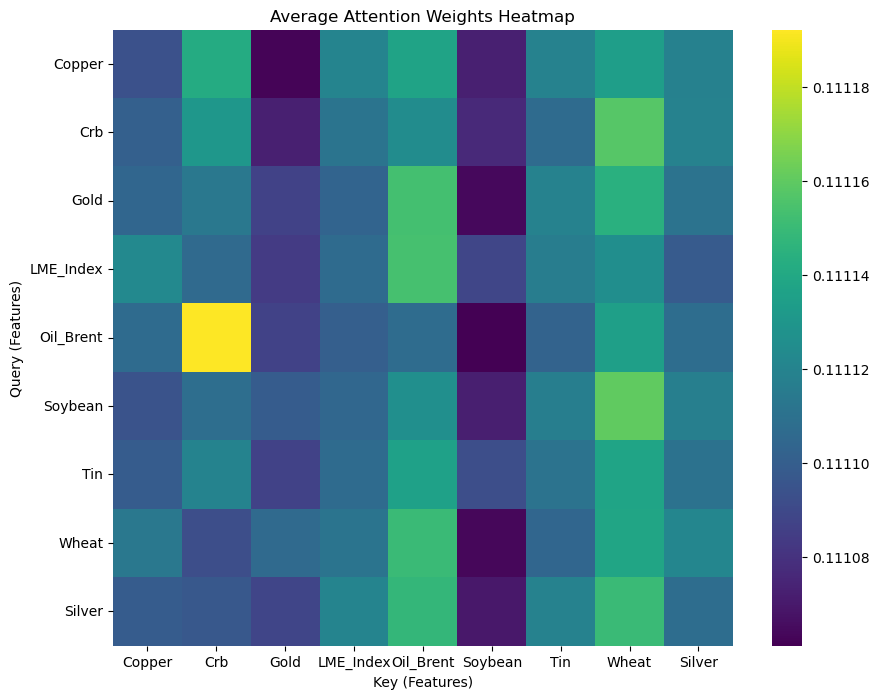
\includegraphics[width=\linewidth]{figures/attention_all_weights.png}
        \caption{All Attention Weights}
        \label{fig:all_attention_weight}
    \end{subfigure}
    \hfill
    \begin{subfigure}[b]{0.48\linewidth}
        \centering
        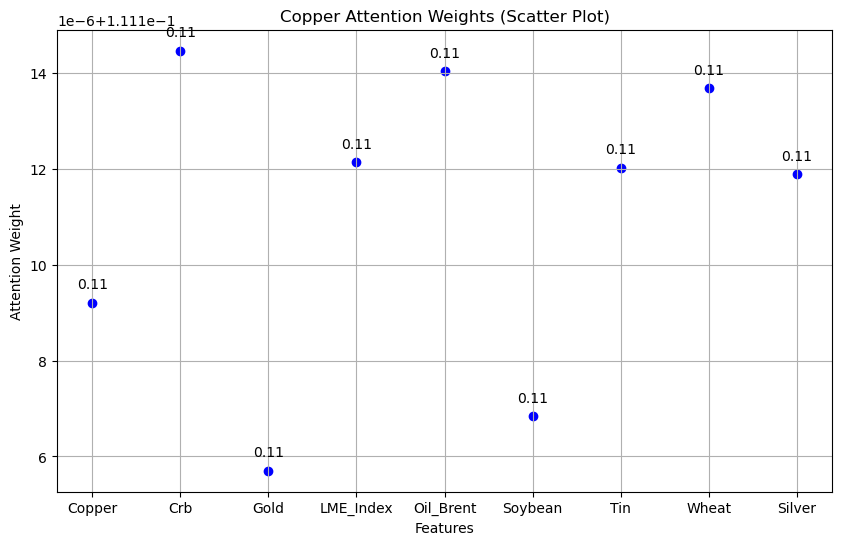
\includegraphics[width=\linewidth]{figures/attention_weights.png}
        \caption{Copper attention weight}
        \label{fig:copper_weight}
    \end{subfigure}
    \caption{Comparison of Attention Weights}
    \label{fig:attention_comparison}
\end{figure}

Depending on the \autoref{fig:attention_comparison}, we can find that Copper prices are closely related to the Commodity Research Bureau Index, oil prices and wheat. The London Metal Exchange Index, tin and silver are next, and gold is the last. I believe this model architecture can be used to analyze other more complex market relationship. As the time period of the training data we use is different, we have the opportunity to use this model to explore relationship between the market factors within the data time.

\subsection{Using BNNs for Capturing Market Randomness}
Bayesian Neural Networks (BNNs) offer a probabilistic approach to modeling everyday distribution, making them well-suited for forecasting in highly uncertain environments like financial markets. BNNs learn distributions on the weights, which allows them to capture the randomness in market data. By sampling from the posterior distribution during inference, BNNs provide predictions that reflect not only the learned trend but also the variability observed in historical data. On the \autoref{fig:bnn_prediction_curve}, we can find that the green area is the 95\% confidence interval of the predicted value. Our average value is very close to the true value, and the confidence interval almost cover the fluctuations of each day. We can think that the model has indeed captured the overall trend and daily random fluctuations, which is much better than Multi-CNN-LSTM-Attention model.

\section{Conclusion}

On the conclusion, to deal with random part issues, we try to use data augmentation with EMD technique to encourage model to learn the trend of the Copper market instead of using today's price as the prediction of the next day. Additionally, Bayesian Neural Networks (BNNs) are really suitable to predict financial market which is a typically random walk model.  It can learn a distribution of copper price, which consider both long term trend and short term randomness.

Looking for \autoref{fig:combined_prediction_curves}, we can find that the result of the next fifth day price is near with exact true value but as what we have said before, there are heavy randomness on the market daily price change. According on the copper price EDA, we can found that the copper price series is very non-stationary and have a obvious trend through all time. If we difference original data and find that it become a noise signal which is a type of random walk. On conclusion, because of the these characteristics of copper price, it is not reasonable to predict exact value on one day but prefer to predict a long term trend. That is why our model is not perform well on real world market even they have achieved high performance on criterion metrics.   

Multi-CNN-LSTM-Attention model compared with BNN-CNN-LSTM model, even though, it perform higher degree on the criterion measurements, I prefer the BNN-CNN-LSTM model as it can capture random information which is align with copper market characteristic. In real world, there are many uncertain and unpredictable factors when predicting financial market. Using BNN-CNN-LSTM model to forecast real financial market can be more robust and flexible. 
\newpage

% References
\bibliographystyle{plain}
\bibliography{references}  % BibTeX references are saved in references.bib

\end{document}          
